
% \subsubsection{Implementar módulo para añadir lugares al sistema}
\subsubsection{Registro de Lugares en el sistema}

Para registrar un \emph{lugar} primeramente se implementó el formulario que se usará para recolectar la información del \emph{lugar}, el formulario fue creado usando \emph{EmberJs} y se lo puede ver en la figura \ref{fig:new_place}. \\

\begin{figure}[H]
     \begin{center}
       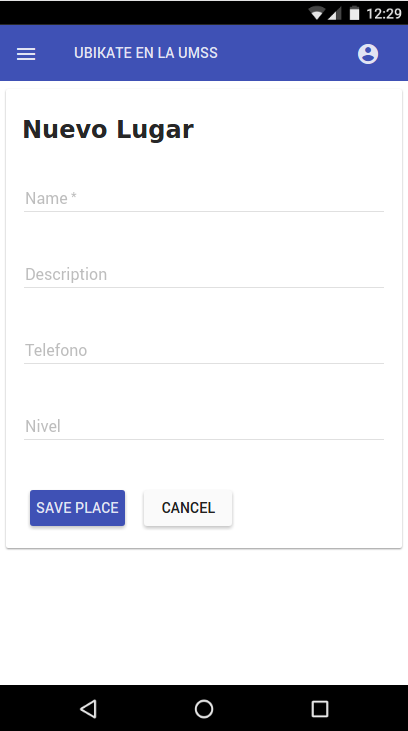
\includegraphics[width=0.3\textwidth]{new_place}

       \caption{Formulario para añadir un nuevo \emph{lugar}.}
       \label{fig:new_place}
       \caption*{Fuente: Elaboración propia.}
     \end{center}
\end{figure}

Posteriormente es necesario crear la petición HTTP desde el controlador de \emph{EmberJS} hacia el API, en el cuerpo de la petición se incluye la posición georeferenciada del celular utilizando el API de Geolocalización de HTML5 usada anteriormente para encontrar la ubicación del usuario, también se incluye el nombre, la descripción, el teléfono y el nivel del \emph{lugar}. En el codigo \ref{new_place_request} se puede ver la implementación de la petición.


% En la figura \ref{fig:new_place} se puede ver el formulario implementado usando \emph{ember-paper}, el cual colecciona los datos que se quieren introducir y se los envía al backend usando una llamada AJAX, como se puede ver en el siguiente código, para crear la petición POST se obtiene las coordenadas actuales del dispositivo móvil además de los datos recolectados del formulario y que con la ayuda de \emph{JQuery} es enviado al API el cual maneja la información recibida y se encarga de insertar los datos en la base de datos.\\

% \newpage
\begin{center}
 \begin{lstlisting}[label=new_place_request,caption=POST request creado en el controlador de \emph{ember}]

   var payload = {
       name: nombre,
       description: descripcion,
       phone: telefono,
       level: nivel,
       lat: latitud,
       lon: longitud
   };

   var url = (ENV.APP.API_HOST || '') + '/api/v1/places/';
   jQuery.post(url, payload).then(
       function(data) {
           var transition = controller.get('transition');
           if (transition) {
               self.transitionTo('places.show');
           } else {
               self.transitionTo('places');
           }
       },
       function(error) {
           controller.set('message', error.responseText);
       }
   );

 \end{lstlisting}
\end{center}

% En esta iteración se implementó la opción de añadir más lugares al sistema, de editarlos y eliminarlos, y la primera tarea es crear las consultas SQL para llevar a cabo las tareas. \\

% por lo que es necesario crear las consultas SQL que insertaran los datos enviados desde el dispositivo móvil al servidor. \\

% Como requisito para insertar un nuevo ``lugar'', se requiere que el usuario esté posicionado en el ``lugar'' ya que se usaran sus coordenadas para posicionar el ``lugar''. Las coordenadas del usuario son obtenidas usando el API de Geolocalización propia de HTML5, usada anteriormente para encontrar la ubicación del usuario \emph{visitante} en la iteración 2.\\

% Posteriormente se necesita implementar el formulario que el usuario usará para insertar los datos del ``lugar'': el nombre, la descripción, el teléfono y el nivel.\\

% Para insertar un ``lugar''  en la base de datos se usó el codigo \ref{new_place}, donde se puede observar la consulta SQL usada, para la cual se necesita capturar la latitud y longitud respectiva donde se encuentra el usuario, además de los datos del ``lugar''.\\

La petición creada es recibida en el API utilizando el \emph{endpoint} RESTful designado para ello, \verb|router.post('/', places.newPlace);|, el \emph{endpoint} se encarga de mandar la información recibida hacia la base de de datos, tomando en cuenta que la posición del lugar es un tipo especial de la base de datos, la latitud y longitud necesitan ser transformadas al momento de insertar el \emph{lugar} en la base de datos, como se muestra en el codigo \ref{cod-new_place_api}.


\begin{center}
 \begin{lstlisting}[label=cod-new_place_api,caption=Insertar un ``lugar'' en la base de datos.]

   router.post('/', places.newPlace);

   var newPlace = (req, res) => {
       var name = req.body.name || '';
       var lat = req.body.lat || '';
       var lon = req.body.lon || '';
       var description = req.body.description || '';
       var phone = req.body.phone || '';
       var level = req.body.level || '';

       let raw = `insert into place (name, geom, description, phone, level)
                  values ('${name}',
                          ST_GeomFromText('POINT(${lon} ${lat})', 3875),
                          '${description}',
                          '${phone}',
                          '${level}'
                         );`;

       Knex.raw(raw)
           .then(function(data) {
               res.json({
                   "message": "Place saved successfully!",
                   "data": data
               });
           })
           .catch(function(error) {
               res.send("Error:", error);
           });
   };

 \end{lstlisting}
\end{center}




% Para la creación de un ``lugar'' es necesario implementar un \emph{endpoint} en el API y siguiendo las convenciones REST se , para que como ya se explicó anteriormente el frontend pueda comunicarse con el backend. \\

% En el API de la aplicación, se implementó un \emph{endpoint} para que pueda manejar los \emph{request} del cliente para añadir un lugar, este \emph{request} es enviado usando el verbo HTTP \emph{POST}, que como ya se explicó es el usado en un REST API para crear objetos. \\

\subsubsection{Edición de la información del Lugar}

Para editar de la información de un lugar se rehusó el formulario ya creado para el registro del mismo, pero populando los campos con la información actual del lugar, el resultado se lo puede ver en la figura \ref{fig:place_edit_form}. \\

\begin{figure}[H]
     \begin{center}
       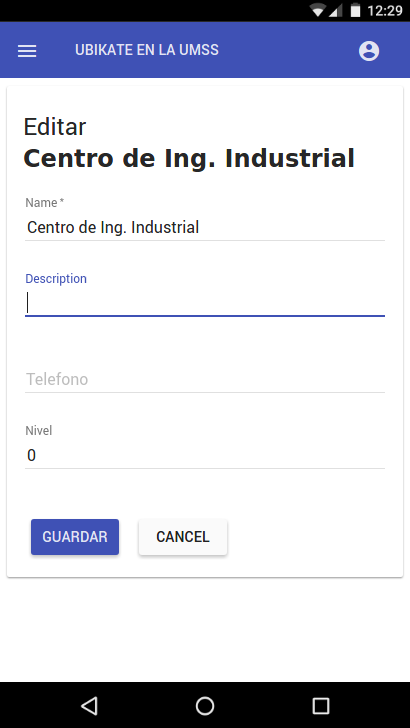
\includegraphics[width=0.3\textwidth]{place_edit_form}

       \caption{Formulario para editar un \emph{lugar}}
       \label{fig:place_edit_form}
       \caption*{Fuente: Elaboración propia.}
     \end{center}
\end{figure}


Los cambios a la información del \emph{lugar} son enviados al API mediante una petición PUT, siguiendo los lineamientos del REST API implementado, esta petición se puede ver en el codigo \ref{cod-edit_place_request}.

\newpage
\begin{center}
 \begin{lstlisting}[label=cod-edit_place_request,caption=Petición HTTP para editar un lugar.]

   router.put('/:id', places.editPlace);

   var body = {
       name: name,
       description: description,
       phone: phone,
       level: level
   };

   var url = (ENV.APP.API_HOST || '') + `/api/v1/places/${id}`;
   jQuery.ajax({
       url: url,
       type: 'put',
       data: body
   }).then(
       function(data) {
           self.transitionTo('places.show', id);
       },
       function(error) {
           controller.set('message', error.responseText);
       }
   );

 \end{lstlisting}
\end{center}

A diferencia del registro del \emph{lugar}, que guarda la posición georeferenciada al momento de registrar el \emph{lugar}, en la edición de los datos no se está tomando en cuenta este dato porque se noto que generalmente cuando se requiere actualizar los datos del \emph{lugar}, el usuario no se encuentra en la posición original del \emph{lugar} y este dato se pierde, corrompiendo la base de datos. Es por esta razón que se decidió que no se actualizará la posición geográfica del \emph{lugar} sin alguna opción explícita que advierta al usuario de las consecuencias de esta acción, pero como tal tarea no se halla dentro de la \emph{historia de usuario} que se esta implementado, se tomo la decisión de realizarla en una futura iteración.








% \subsubsection{Eliminar un lugar}

% Una vez implementado la lógica para añadir un ``lugar'', se implementó los módulos para poder eliminar el ``lugar'', para esto se añadió un botón en la lista de lugares, el cual despliega un mensaje de advertencia al usuario de que está por eliminar un ``lugar'' y que la acción es irreversible, por lo tanto este botón sólo está disponible para un usuario \emph{administrador}. \\
%
% La verbo  HTTP \emph{DELETE} es el que de acuerdo a la implementación del API REST es el adecuado para eliminar un lugar, por lo tanto es el que se usó en la aplicación. En el codigo \ref{delete_place_enpoint} se puede observar el \emph{endpoint} implementado en el API que se encarga de manejar las peticiones \emph{DELETE} creando una consulta SQL que elimina el lugar de la base de datos.\\
%
% \begin{center}
%   \begin{lstlisting}[label=delete_place_enpoint,caption=DELETE request elimina un lugar.]
%
%     router.delete('/:id', places.deletePlace);
%
%     var deletePlace = (req, res) => {
%         var id = req.params.id;
%
%         Place.forge({
%             gid: id
%         })
%         .destroy()
%         .then(function(model) {
%             res.json({
%                 "message": "Place deleted successfully!"
%             });
%         })
%         .catch(function(err) {
%             res.status(500);
%         });
%     };
%
%   \end{lstlisting}
% \end{center}
%
% En el anterior codigo se puede apreciar la bondad de usar un manejador de bases de datos como \emph{Bookshelf} ya que usando el método \verb|destroy()|, se encarga automáticamente de crear la consulta SQL para eliminar una tupla de la base de datos.\\
